% !TeX program = XeLaTeX
% !TeX root=./main.tex
% Edit by:
\setlength{\abovedisplayskip}{5pt}
\setlength{\belowdisplayskip}{5pt}

\chapter{多维随机变量及其分布}\label{cha:3}
在有些随机现象中, 对每个样本点 $\omega$ 只用一个随机变量去描述是不够的, 
譬如要研究儿童的生长发育情况, 仅研究儿童的身高 $X(\omega)$ 或仅研究其体重 $Y(\omega)$都是片面的, 
有必要把 $X(\omega)$ 和 $Y(\omega)$ 作为一个整体来考虑, 讨论它们总体变化的统计规律性, 
进一步可以讨论 $X(\omega)$ 与 $Y(\omega)$ 之间的关系, 在有些随机现象中, 甚至要同时研究二个以上随机变量. 

如何来研究多维随机变量的统计规律性呢, 仿一维随机变量, 我们先研究联合分布函数, 
然后研究离散随机变量的联合分布列、连续随机变量的联合密度函数. 

\section{多维随机变量及其联合分布}\label{sec:3.1}

\subsection{多维随机变量}\label{ssec:3.1.1}
下面我们先给出 $n$ 维随机变量的定义. 
\begin{definition}{随机变量}{3.1.1}
	如果 $X_1(\omega),X_2(\omega),\ldots,X_n(\omega)$ 是定义在同一
	样本空间 $\Omega=\left\{\omega\right\}$ 上的 $n$ 个随机变量, 则称
	\[
	X(\omega)=(X_1(\omega),X_2(\omega),\ldots,X_n(\omega))
	\]
	为 $n$ 维(或 $n$ 元)\textbf{随机变量}\index{S!随机变量}或\textbf{随机向量}\index{S!随机向量}. 
\end{definition}
注意, 多维随机变量的关键是定义在同一样本空间上, 对于不同样本空间上的两个随机变量, 我们只能在
乘积空间 $\Omega_1\times \Omega_2=\left\{(\omega_1,\omega_2);\omega_1 \in \Omega_1,\omega_2 \in \Omega_2 \right\}$ 上讨论, 
 这要用到更多的工具, 本章将不涉及这类问题. 
      
 在实际问题中, 多维随机变量的情况是经常会遇到的臂如
  \begin{itemize}
  	\item 在研究四岁至六岁儿童的生长发育情况时, 我们感兴趣于每个儿童(样本点 $\omega$ )的身高 $X_1(\omega)$ 
  	和体重 $X_2(\omega)$ . 这里 $(X_1(\omega),X_2(\omega))$是一个二维随机变量. 
  	\item 在研究每个家庭的支出情况时, 我们感兴趣于每个家庭(样本点 $\omega$ )的衣食住行四个方面, 
  	若用 $X_1(\omega),X_2(\omega),X_3(\omega),X_4(\omega)$ 分别表示衣食住行的花费占其家庭总收人的百分比, 
  	则 $X_1(\omega),X_2(\omega),X_3(\omega),X_4(\omega)$ 就是一个四维随机变量. 
  \end{itemize}

  \subsection{联合分布函数}\label{3.1.2}
  \begin{definition}{联合分布函数}{3.1.2}
  	对任意的 $n$ 个实数 $x_1,x_2,\ldots,x_n ,$ 则 $n$ 个事件 $\{X_1\leq x_1\},\{X_2 \leq x_2\},\ldots,\{X_n\leq x_n\}$ 同时发生的概率
    \begin{equation}
    	F\left(x_{1}, x_{2}, \cdots, x_{n}\right)=P\left(X_{1} \leq x_{1}, X_{2} \leq x_{2}, \ldots, X_{n} \leq x_{n}\right)\label{eq:3.1.1}
    \end{equation}
	称为 $n$ 维随机变量 $(X_1,X_2,\ldots,X_n)$ 的\textbf{联合分布函数}\index{L!联合分布函数}. 
  \end{definition}
   本章主要研究二维随机变量, 二维以上的情况可类似进行. 

   在二维随机变量 $(X,Y)$ 场合, 联合分布函数 $F(x,y)=P(X\leq x,Y\leq y)$ 是事件 $\{X\leq x\}$ 与 $\{Y \leq y\}$ 同时发生(交)的概率. 
   如果将二维随机变量 $(X,Y)$ 看成是平面上随机点的坐标, 那么联合分布函数 $F(x,y)$ 在 $(x,y)$ 处的函数值就是随机点 $(X, Y)$ 落在
   以 $(x,y)$ 为右上角的无穷矩形内的概率, 见图~\ref{fig:3.1.1} .
   \begin{figure}[htbp]
   	\centering
   	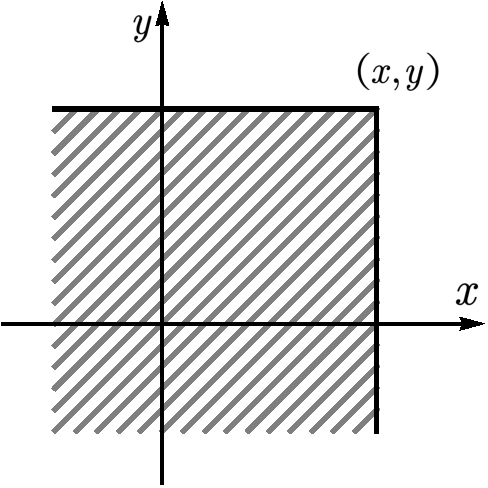
\includegraphics[width=0.4\textwidth]{fig3-1-1.pdf}
   	\caption{联合分布函数示意图}\label{fig:3.1.1}
   \end{figure}
   \begin{theorem}{}{3.1.1}
   	任一二维联合分布函数 $F(x,y)$ 必具有如下四条基本性质: 
    \begin{enumerate}
    	\item \textbf{单调性}\quad $F(x,y)$ 分别对 $x$ 或 $y$ 是单调不减的,即
    	\begin{itemize}
    		\item 当 $x_1<x_2$ 时, 有 $F(x_1,y)\leq F(x_2,y)$.
    		\item 当 $y_1<y_2$ 时, 有 $F(x,y_1)\leq F(x,y_2)$. 
    	\end{itemize}
    	\item \textbf{有界性}\quad 对任意的 $x$ 和 $y$, 有 $0\leq F(x,y) \leq 1$, 且
    	\begin{align*}
    		&F(-\infty,y)=\lim_{x\to -\infty}F(x,y)=0,	&\hspace*{3cm} \\
    		&F(x,-\infty)=\lim_{y\to -\infty}F(x,y)=0,	&\\
    		&F(+\infty,+\infty)=\lim_{x,y\to +\infty}(x,y)=1.&
    	\end{align*}
    	\item \textbf{右连续性}\quad  对每个变量都是右连续的,即
    		\begin{align*} 
    			F(x+0, y) &=F(x, y), &\hspace*{3cm} \\ 
    			F(x, y+0) &=F(x, y). &
    		\end{align*}
    	\item \textbf{非负性}\quad 对任意的 $a<b,c<d$ 有
    		\begin{equation*}
    		 	P(a<X \leq b, c<Y \leq d)= F(b, d)-F(a, d)-F(b, c)+ F(a, c) \geq 0 .
    		\end{equation*}
    		\begin{proof}
    			\begin{enumerate}
    				\item  因为当 $x_1<x_2$ 时, 有 $\{X_1\leq x_1\} \subset \{X_2 \leq x_2\}$, 所以对任意给定的 $y$ 有
    				\[
    				 	\left\{X \leq x_{1}, Y \leq y\right\} \subseteq \{ X \leq x_{2}, Y \leq y \},
    				\]
    				由此可得
    				\[
    				 	F\left(x_{1}, y\right)=P\left(X \leq x_{1}, Y \leq y\right) \leq 
    				 	P\left(X \leq x_{2}, Y \leq y\right)=F\left(x_{2}, y\right),
    				\]
    				即 $F(x,y)$ 关于 $x$ 是单调不减的, 同理可证 $F(x,y)$ 关于 $y$ 是单调不减的.
    				\item 由概率的性质可知 $0\leq F(x,y) \leq 1$. 又因为对任意的正整数 $n$ 有
    				\begin{align*}
    					&\lim_{x\to -\infty}\{X\leq x\}=\lim_{n\to +\infty}\bigcap_{m=1}^n \{X\leq -m\}=\varnothing,	\\
    					&\lim_{x\to +\infty}\{X\leq x\}=\lim_{n\to +\infty}\bigcup_{m=1}^n\{X\leq m\}=\Omega,
    				\end{align*}
    				对 $Y \leq y$ 也类似可得. 再由概率的连续性, 就可得
    				\[
    				 	F(-\infty, y)=F(x,-\infty)=0; \quad F(+\infty,+\infty)=1.
    				\]
    				\item 固定 $y$, 仿一维分布函数右连续的证明, 就可得知 $F(x, y)$ 关于 $x$ 是右连续的. 同样固定 $x$ 可
    				证得 $F(x,y)$ 关于 $y$ 是右连续的.
        			\item 只需证
        			\[
        			 	P(a<X \leq b, c<Y \leq d)=F(b, d)-F(a, d)-F(b, c)+F(a, c).
        			\]
        			为此记 ( 见图~\ref{fig:3.1.2} )
        			\[
        			 	A=\{X \leqslant a\}, \quad B=\{ X \leqslant b \}, \quad C=\{Y \leqslant c\}, \quad D=\{Y \leqslant d\},
        			\]
        			考虑到
        			\[
        			 	\{ a<X \leqslant b \}=B-A=B \cap \overline{A}, \quad\{c<Y \leqslant d\}=D-C=D \cap \overline{C},
        			\]
        			且 $A \subset B, C\subset D,$ 由此可得
        			\begin{align*}
        				 0 & \leqslant P(a<X \leqslant b, c<Y \leqslant d) \\ 
        				 &=P(B \cap \overline{A} \cap D \cap \overline{C}) \\ 
        				 &=P(B D-(A \cup C)) \\ 
        				 &=P(B D)-P(A B D \cup B C D) \\ 
        				 &=P(B D)-P(A D \cup B C) \\ 
        				 &=P(B D)-P(A D)-P(B C)+P(A B C D) \\ 
        				 &=P(B D)-P(A D)-P(B C)+P(A C ) \\ 
        				 &=P(B D)-P(A D)-P(B C)+P(A B C D) \\ 
        				 &=F(b, d)-F(a, d)-F(b, c)+F(a, c). 
        			\end{align*}
    			\end{enumerate}
    		\end{proof}
    \end{enumerate}
   \end{theorem}
   \begin{figure}[htbp]
   	\centering
   	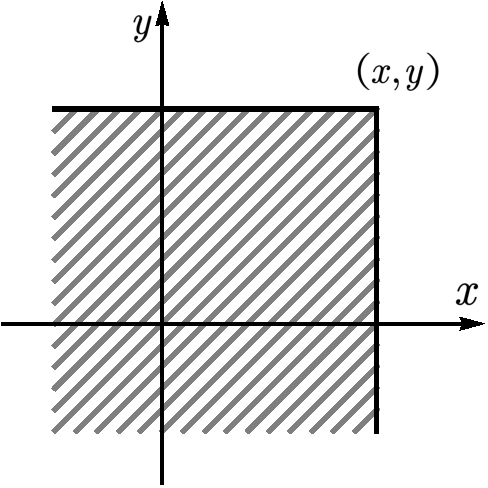
\includegraphics[width=0.4\textwidth]{fig3-1-1.pdf}
   	\caption{二维随机变量 $(X,Y)$ 落在矩形中的情况}\label{fig:3.1.2}
   \end{figure}